\textbf{ID:} UC05 (Edit Event) \\
\textbf{Scope:} CS Automated Information Timeline \\
\textbf{Level:} User Goal \\
\textbf{Primary Actor:} Faculty \\
\textbf{Stakeholders and Interests:}
\begin{itemize}
    \item Audience: Wants to view up-to-date information about events in the CS Department
    \item Faculty: Wants the ability to provide updated information on events they submitted
    \item Office Manager: Wants to display accurate event information on the calendar on the Lobby TV
    \item Admin/Reviewer: Wants to update previously approved events with up-to-date information provided by the Faculty who submitted those events
\end{itemize}
\textbf{Preconditions:} Faculty created an event (UC04) and submitted it for review (UC08). Admin/Reviewer reviewed the event (UC09) and approved. Admin/Reviewer is identified and authenticated in the system. Faculty is identified and authenticated in the system and is viewing the event calendar (UC03). \\
\textbf{Postconditions:} Event status is in a proposed state. \\
\textbf{Main Success Scenario:}
\begin{enumerate}
    \item Faculty clicks the ``View My Events'' link on the event calendar page.
    \item System returns a list of existing events authored by Faculty that have been approved.
    \item Faculty selects the event they wish to edit from the returned list of their previously approved events.
    \item System returns the event page for the selected event.
    \item Faculty clicks the “Edit This Event” button on the event page.
    \item Faculty enters the updated event information into the submission form:
          \begin{itemize}
              \item Event date
              \item Event time
              \item Event description
          \end{itemize}
    \item Faculty submits the updated event information for Admin/Reviewer review.
    \item System provides Faculty with a submission confirmation message.
\end{enumerate}
\textbf{Extensions (or Alternate Flows):} \\
3-4a. Faculty begins editing the event, then decides not to submit the updates for review:
\begin{enumerate}
    \item Upon leaving the web page, any changes to event date, time, or description entered into the submission form are erased.
    \item Selected event remains unchanged in the system.
\end{enumerate}
3b. Faculty does not see the event they wish to edit in the returned list because the event has not yet been approved by the Admin/Reviewer:
\begin{enumerate}
    \item Faculty must wait for approval from Admin/Reviewer on the original event before the event is eligible for editing.
\end{enumerate}
\textbf{Special Requirements:} None \\
\textbf{Technology and Data Variations List:} \\
4a. Date input is required in the format MM/DD/YYYY. \\
4b. Time input is required in the Standard Time format in the Central Time Zone. \\
\textbf{Frequency of Occurrence:} Could be nearly continuous if Admin/Reviewer also reviews edited events and approves them (UC09) nearly continuously. \\
\textbf{Open Issues:} None \\

\begin{figure}[H]
    \centering
    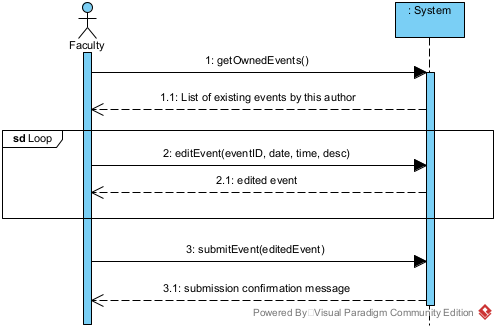
\includegraphics[width=0.8\textwidth]{images/SSD-UC05-EditEvent.png}
    \centering
    \caption{System Sequence Diagram: Edit Event}
\end{figure}

\textbf{Operation:} getOwnedEvents() \\
\textbf{Cross-References:} UC05 (Edit Event), UC06 (Delete Event), UC07 (View Event) \\
\textbf{Pre-conditions:} Event object has been created. Event has been associated with Faculty. Event attribute status is set to approved. \\
\textbf{Post-conditions:} None. \\

\textbf{Operation:} editEvent(eventID, date, time, desc) \\
\textbf{Cross-References:} UC05 (Edit Event) \\
\textbf{Pre-conditions:}
\begin{itemize}
    \item Event object has been created.
    \item Event attribute status is set to approved.
    \item Event has been associated with Faculty.
\end{itemize}
\textbf{Post-conditions:} editedEvent has been created.
\begin{itemize}
    \item editedEvent object has been created.
    \item editedEvent attributes (date, time, desc) have been updated.
    \item editedEvent has been associated with Faculty.
\end{itemize}

\textbf{Operation:} submitEvent(editedEvent) \\
\textbf{Cross-References:} UC05 (Edit Event) \\
\textbf{Pre-conditions:}
\begin{itemize}
    \item editedEvent object has been created.
    \item editedEvent attributes (date, time, desc) have been updated.
    \item editedEvent has been associated with Faculty.
\end{itemize}
\textbf{Post-conditions:}
\begin{itemize}
    \item Notification object is created.
    \item Notification object is associated with editedEvent, Faculty, and Admin/Reviewer.
\end{itemize}